%\documentclass[draft,a4paper,DIVcalc,abstract,english]{scrartcl}
\documentclass[a4paper,DIVcalc,abstract,english]{scrartcl}
\usepackage[utf8]{inputenc}
\usepackage[T1]{fontenc}
\usepackage{babel}
\usepackage{graphicx}
\usepackage{booktabs}
\usepackage{todonotes}
\usepackage[binary-units=true]{siunitx}
	\DeclareSIUnit\Molar{\textsc{m}}
	\sisetup{separate-uncertainty}
\usepackage{textcomp} % to suppress warnings from microtype
\usepackage{svn-multi}
\usepackage{subfig}
\usepackage{fancyhdr}
\usepackage{tikz}
\usepackage{pgfplots}
	\pgfplotsset{compat=newest}
\usepackage[square,sort&compress]{natbib} % add "numbers" for the way the journal wants it
\usepackage{scrtime}
\usepackage{xspace}
\usepackage[autostyle=true]{csquotes}
%%%%%%%%%%%% Für Johannes %%%%%%%%%%%%
\usepackage{setspace} % Change spacing
	%\singlespacing
	\onehalfspacing
	%\doublespacing
\usepackage[none]{hyphenat}\raggedright % No hyphenation, but ugly output
\setlength{\parindent}{10pt}
%%%%%%%%%%%% Für Johannes %%%%%%%%%%%%
\usepackage{microtype}
\usepackage[backref]{hyperref}

% Header
\title{Visualization and stereological characterization of individual rat lung acini by high resolution X-ray tomographic microscopy}

\author{%
	David Haberthür\footremember{psi}{Swiss Light Source, Paul Scherrer Institut, Villigen, Switzerland}\ \footremember{ana}{Institute of Anatomy, University of Bern, Switzerland}%
	\and Sébastien F. Barré\footrecall{ana}% \footremember{gcb}{Graduate School for Cellular and Biomedical Sciences, University of Bern, Switzerland}%
	\and Stefan A. Tschanz\footrecall{ana}%
	\and Evelyne Yao\footrecall{ana}%
	\and Marco Stampanoni\footrecall{psi} \footremember{eth}{Institute for Biomedical Engineering, Swiss Federal Institute of Technology and University of Zürich, Switzerland}%
	\and Johannes C. Schittny\footrecall{ana}\ \footremember{contact}{Corresponding Author. Prof.\ Dr.\ Johannes C.\ Schittny, Institute of Anatomy, University of Bern, Baltzerstrasse 2, CH-3012 Bern, +41 31 631 46 35, \href{mailto:schittny@ana.unibe.ch}{schittny@ana.unibe.ch}}%
	}
 
% Subversion Information
\svnidlong
{$HeadURL$}
{$LastChangedDate$}
{$LastChangedRevision$}
{$LastChangedBy$}
\svnid{$Id$}

% Setup
\newcommand{\imsize}{\linewidth}
\newlength\imagewidth		% needed for scale bars
\newlength\imagescale		% ditto
\newcommand{\footremember}[2]{\footnote{#2}\newcounter{#1}\setcounter{#1}{\value{footnote}}}
\newcommand{\footrecall}[1]{\footnotemark[\value{#1}]}
\newcommand{\superscript}[1]{\ensuremath{^{\textrm{#1}}}}
\newcommand{\subscript}[1]{\ensuremath{_{\textrm{#1}}}}
\newcommand{\ie}{i.\,e.\ }
\newcommand{\eg}{e.\,g.\ }
\newcommand{\subfigureautorefname}{\figureautorefname} % make \autoref work with \subfloat
\pagestyle{fancy}
\fancyhead[R]{\thepage}
\fancyhead[L]{Stereological characterization of individual acini}
\fancyfoot[C]{\href{\svnkw{HeadURL}}{SVN-Revision \svnkw{LastChangedRevision}}, typeset on \today\ at \thistime}

% Data
\newcommand{\shrinkagefactor}{0.61} % Shrinkagefactor used for the calculation
\newcommand{\numberofacini}{43}
\newcommand{\numberofaciniB}{24}
\newcommand{\numberofaciniD}{10}
\newcommand{\numberofaciniE}{9}
\newcommand{\numberofoutliers}{4} % Number of Outliers removed
\newcommand{\biggerthan}{2} % Outliers bigger/smaller than mean +- BiggerThan * STD have been removed

\newcommand{\totalnumberofaciniB}{9197}
\newcommand{\totalnumberofaciniD}{5257}
\newcommand{\totalnumberofaciniE}{4845}
\newcommand{\meantotalnumberofacini}{6433}
\newcommand{\meantotalnumberofaciniSTD}{1962} % add "ddof=1" to get the same STD as with "=STDEV()" in Excel
\newcommand{\meantotalnumberofacinirounded}{6400}

\newcommand{\totalnumberofaciniBVariant}{6052}
\newcommand{\totalnumberofaciniDVariant}{6066}
\newcommand{\totalnumberofaciniEVariant}{4292}
\newcommand{\meantotalnumberofaciniVariant}{5470}
\newcommand{\meantotalnumberofaciniSTDVariant}{833} % add "ddof=1" to get the same STD as with "=STDEV()" in Excel

\newcommand{\acinarvolumeB}{6.929e-04} % cm^3
\newcommand{\acinarvolumeD}{1.361e-03} % cm^3
\newcommand{\acinarvolumeE}{1.389e-03} % cm^3
\newcommand{\meanacinarvolume}{1.148e-03} % cm^3, (mean acinar volume)
\newcommand{\std}{3.219e-04} % (Standard deviation of acinar volumes), add "ddof=1" to get the same STD as with "=STDEV()" in Excel

\newcommand{\numberofalveoliB}{6505}
\newcommand{\numberofalveoliD}{9330}
\newcommand{\numberofalveoliE}{12750}
\newcommand{\meannumberofalveoli}{8470} % (Mean number of alveoli per acinus)
\newcommand{\difference}{2.661} % X times bigger (acinar volumes STEPanizer/MeVisLab-volumes)

\newcommand{\acinarsurfaceB}{0.458} % cm^2
\newcommand{\acinarsurfaceD}{0.69} % cm^2
\newcommand{\acinarsurfaceE}{1.069} % cm^2
\newcommand{\meanacinarsurface}{0.739} % cm^2

\newcommand{\airspacesurfaceB}{4214} % cm^2
\newcommand{\airspacesurfaceD}{3628} % cm^2
\newcommand{\airspacesurfaceE}{5177} % cm^2
\newcommand{\meanairspacesurface}{4340} % cm^2

\newcommand{\airspacedifference}{1.848} % times

\begin{document}
%\setcounter{secnumdepth}{-1} % No section numbering, please!
\renewcommand{\subsectionautorefname}{\sectionautorefname} % useful for \autoref
\renewcommand{\subsubsectionautorefname}{\sectionautorefname} % useful for \autoref
\maketitle
\begin{center}
\vfill
Typeset on \today\ at \thistime\ from Rev \svnkw{LastChangedRevision} (\svnday.\svnmonth.\svnyear\ \svnhour:\svnminute)
\vfill
To be submitted to the \emph{\href{http://jap.physiology.org/}{Journal of Applied Physiology}}, \emph{Innovative Techniques}, thus formatted according to \href{http://www.the-aps.org/mm/Publications/Preparing-Your-Manuscript#file_format}{their guidelines}
\vfill
\end{center}
\clearpage

\section*{Contributions}
\begin{itemize}
	\item David Haberthür performed data acquisition, estimated acinar volumes and surfaces, designed and performed analysis of data and wrote the manuscript.
	\item Sébastien F. Barré performed data acquisition and contributed to analysis of data.
	\item Stefan A. Tschanz obtained the samples and contributed to stereological analysis.
	\item Evelyne Yao prepared the samples and estimated alveolar numbers of the acini.
	\item Marco Stampanoni designed the beamline and contributed to writing.
	\item Johannes C. Schittny conceived and designed the study, obtained the samples, performed the data acquisition and contributed to writing.
\end{itemize}

\section*{Running title}
See page header

\section*{Keywords}
\begin{itemize}
	\item synchrotron radiation 
	\item microCT
	\item (number of) alveoli
\end{itemize}
\clearpage

\begin{abstract}
The small trees of gas-exchanging pulmonary airways which are fed by the most distal purely conducting airways are called acini and represent the functional gas-exchanging unit.
The three-dimensional architecture of the acini has a strong influence on ventilation and particle deposition.
Due to the difficulty to identify single acini in lung sections the knowledge about the number of acini and their individual biological parameters like volume, surface area, and number of alveoli per acinus are limited.
We developed a method to extracted individual pulmonary acini from lung samples imaged by high-resolution X-ray tomographic microscopy and estimated their volume, surface area and number of alveoli.
Rat acini were isolated by semi-automatically closing the airway at the transition from conducting to gas-exchanging airways.
We estimated a mean acinar volume of \SI{\meanacinarvolume}{\centi\meter\cubed}, a mean acinar surface area of \SI{\meanacinarsurface}{\centi\meter\squared}, and a mean of \meannumberofalveoli\xspace alveoli per acinus.
Assuming that the acini are similarly sized throughout different regions of the lung, we calculated that a rat lung contains roughly \meantotalnumberofacinirounded\xspace acini.
We conclude that our novel approach is well suited to characterize acini in healthy, diseased, or transgenic lungs of different species including humans.
Our proposed method of analyzing single ventilatory units of the mammalian lung allows for the first time to extract biological parameters of single acini which cannot be extracted from classic physical sections.
\end{abstract}
\clearpage

\section{Introduction}
\subsection{Lung structure and the acini}
The airway structure of the mammalian lung is formed from largely dichotomous branches~\citep{Weibel1991} starting from the trachea.
With increasing depth into the airway tree, the diameter of the airways is reduced.
The pipe-like purely conducting airways begin with the bronchi, which are subdivided into several generations of bronchioles, which in turn are subdivided into terminal bronchioles.
The following transitory bronchioles mark the beginning of the gas-exchange region in the human lung, while in rat lungs this region is formed by the transitory bronchioles, which are tube-like structures covered with single alveoli.

The change between purely conducting and gas-exchanging airways is identified by changes in the airway wall structure---alveolar outpouchings---and in the airway epithelium (see \autoref{fig:ManholeCoverExplanation}).
After this point, the so-called acinar airways and all the following airspace form one functional lung unit, the so-called acinus.
One acinus is composed of an alveolar duct leading into multiple saccules covered by alveoli corresponding to the terminal end of the airway tree~\citep{Schittny2007a}.

The lung structure can be estimated using stereology, as described by \citet{Hsia2010}.
Such an analysis is generally based on two-dimensional sections of the sample, thus the extracted information is a two-dimensional description \blockquote[\citet{Tschanz2002}]{of the parenchymal air space geometry and, due to geometric laws, it is not allowed to extrapolate these two-dimensional statements directly to three-dimensional structures}.
With stereological methods it is possible to extract global volume information, but it is not easily feasible to extract such information from a functional subunit of an organ like the acini in the lung, since it cannot easily be assessed which detail on one microscopy slide belongs to which functional unit in the three-dimensional space.

\subsection{Motivation}
Due a restricted availability of high resolution three-dimensional imaging methods the knowledge about the development of the ventilatory functional unit of the lung is limited.
These functional units of the lung parenchyma are the so-called pulmonary acini, which correspond to the gas-exchange volume in the lung which is ventilated by the most distal generation of purely conducting bronchioles~\citep{Rodriguez1987}.

Extracting large amounts of single acini from physical sections of lung tissue for analyzing the acinar volume is extremely time-consuming.
\citet{Woodward2005} achieved three-dimensional reconstructions of three adult duck lungs using intense manual effort to trace serial sections of the tissue.
\citet{Rodriguez1987} \blockquote{first attempted serial-section reconstructions but realized the limitations of this very tedious although precise method} and finally switched to casting of airways with silicon to assess the acini in rat and rabbits. They analyzed acini of one animal for each species.

\citet{Mercer1987a} manually traced several acini on photographs of serial step sections with a thickness of \SI{3}{\micro\meter} each.
Due to the substantial effort for relating each alveolus to a ventilatory unit, \citeauthor{Mercer1987a} performed such a tracing for \blockquote{only a few} undefined number of cases.

This manuscript describes a method to isolate and analyze single acini from large synchrotron radiation based tomographic microscopy datasets and to stereologically analyze biological parameters of those single functional units of the mammalian lung.
Since tomographic imaging of the lung tissue preserves the three-dimensional structure, single slices from the images can be easily extracted and be used for precise stereological analysis, e.g. the volume, surface area, and number of alveoli per acinus.

In addition to three-dimensional volume analysis through segmentation and voxel counting in a visualization software we performed standard stereological analysis~\citep{Hsia2010} to compare our results with both other results~\citep{Rodriguez1987,Tschanz2003,Mercer1987a}.

The presented method can isolate single functional lung units, mark their extent on virtual two-dimensional slices and thus, for a first time make it possible to perform a stereological characterization of individual acini in the mammalian lung.

\section{Materials and Methods}
\label{sec:materials and methods}
\subsection{Rat lung samples}
Three 60 days old Sprague-Dawley rats were deeply anesthetized with a mixture of %
\SI{0.5}{\milli\gram\per\milli\litre} acetylpromazine, %
\SI{5}{\milli\gram\per\milli\litre} xylazine and %
\SI{50}{\milli\gram\per\milli\litre} ketamine in %
\SI{0.9}{\percent} NaCl at \SIrange{1.5}{2.5}{\micro\litre} per \si{\gram} body weight.
The lungs of the animals were instilled with \SI{2.5}{\percent} glutaraldehyde in \SI{0.03}{\milli\Molar} potassium-phosphate buffer (pH 7.4) at a constant pressure of \SI{20}{\centi\meter} water column.
At this pressure, the rat lung reaches its mid-respiratory volume~\citep{Schittny1998}.
After instillation the lung was removed from the chest cavity and the pressure was maintained during fixation in order to prevent a recoiling of the lung~\citep{Mund2008}.

After fixation, the samples were prepared for tomographic imaging by post-fixation with \SI{1}{\percent} osmium acetate and staining with \SI{4}{\percent} uranyl acetate to increase the x-ray absorption contrast.
Using Histoclear (Merck KGaA, Darmstadt, Germany) as an intermedium the samples were dehydrated in a graded series of ethanol and embedded in paraffin prior to mounting them onto standard scanning electron microscopy sample holders (PLANO GmbH, Wetzlar, Germany) with paraffin~\citep{Tsuda2008}.

The handling of animals before and during the experiments as well as the experiments themselves were approved and supervised by the Swiss Agency for the Environment, Forests and Landscape and the Veterinary Service of the Canton of Bern, Switzerland.

\subsection{Tomographic data acquisition}
Tomographic imaging was performed at the \href{http://www.psi.ch/sls/tomcat/}{TOMCAT beamline}~\citep{Stampanoni2006a} of the \href{http://www.psi.ch/sls/}{Swiss Light Source} at the \href{http://www.psi.ch/}{Paul Scherrer Institute} in Villigen, Switzerland.
The samples were scanned at an x-ray energy of \SI{20.0}{\kilo\electronvolt} and x-rays were converted into visible light by either a \SI{20}{\micro\meter} thick LuAG:Ce or \SI{18}{\micro\meter} thick YAG:Ce scintillator screen (both \href{http://www.crytur.cz/}{Crytur Ltd.}, Turnov, Czech Republic), depending on the date of experiment.
The visible light was magnified using a 10\(\times\) magnifying, diffraction limited microscope optics and recorded with a 2048\(\times\)2048 pixel CCD camera (\href{http://www.pco.de/sensitive-cameras/pco2000/}{pco.2000}, \href{http://www.pco.de/}{PCO AG}, Kelheim, Germany) with \SI{14}{\bit} dynamic range operated in 2\(\times\)2 binning mode.
As a result, the voxel size was \SI{1.48}{\micro\meter} and the exposure time was between \SIrange{160}{200}{\milli\second}.

Alveolar septa in rats have a mean thickness of \SIrange{5}{10}{\micro\meter} (calculated from data by \citet{Burri1974}).
To unambiguously segment the alveolar septa in our datasets, a resolution of  about two microns was required.
To extract a large amount of single acini, we needed to acquire high resolution tomographic scans covering large volume.
Since our samples were larger than the classic field of view of TOMCAT at the aforementioned optical properties (1.52\(\times\)1.52\(\times\)\SI{1.52}{\milli\meter}) we used the so-called wide field scanning method~\citep{Haberthuer2010a}, where three independently acquired tomographic scans perpendicular to the rotation axis of the sample are merged to cover the desired field of view.
Additionally, several wide field scans were stacked parallel to the rotation axis of the sample.
The resulting tomographic datasets covered a field of view of approximately 4.5\(\times\)4.5\(\times\)\SI{4.5}{\milli\meter\cubed} (3000\(\times\)3000\(\times\)3072 voxels at \SI{1.48}{\micro\meter} side length).

\subsection{Visualization and Extraction of Acini}
The tomographic datasets of the sample were three-dimensionally analyzed and visualized using \href{http://mevislab.de}{MeVisLab} (Version 2.1 (2010-07-26 Release), MeVis Medical Solutions AG and Fraunhofer MEVIS -- Institute for Medical Image Computing, Bremen, Germany)~\citep{Bitter2007}.
The analysis and visualizations have been performed using a Dell Precision T7500 work station (\SI{24}{\giga\byte} RAM, Intel Xeon CPU X5550 at \SI{2.66}{\giga\hertz}, Windows 7 Professional \SI{64}{\bit}).

The tomographic datasets obtained at TOMCAT were converted from a stack of TIFF-files to the native GVR format of MeVisLab, a multi-resolution \href{https://secure.wikimedia.org/wikipedia/en/w/index.php?title=Octree&oldid=409131920}{octree}-based image format.
This permitted us to easily switch between resolutions in the dataset to interactively perform the visualization and preliminary analysis on a lower resolution prior to the final analysis on full resolution datasets.
Inside MeVisLab, we developed a graphical user interface (GUI) using the MeVisLab Definition Language to define regions of interest in the dataset, to isolate single acini and extract them from the tomographic dataset for subsequent verification.
With the same GUI we visualized the extracted acini in 3D, calculated their volume and exported a three-dimensional dataset of each acinus in \href{http://en.wikipedia.org/w/index.php?title=DICOM&oldid=511155074}{DICOM}-format for further (stereological) analysis.

\subsubsection{Manhole Covers}
\label{sec:manhole covers}
Airway segments were segmented using a grey-level threshold based region growing algorithm~\citep{Zucker1976}.
A seed point for the region growing algorithm was manually defined inside the conducting airways on one of the most proximal slices of the dataset.
As a result the tree was composed of both conducting and gas-exchanging airways.
Using segmentation stoppers dubbed manhole covers, single acini were isolated from each segmented tree of airways until it was subdivided into purely conducting airways and multiple adjacent separated acini (\autoref{fig:ManholeCoverExplanation} and \ref{fig:workflow}).

Manhole covers were implemented using a \href{http://www.mevis-research.de/cgi-bin/discus/board-auth.cgi?lm=1282233250&file=/839/11760.html}{custom MeVisLab module (\emph{XMarkerClipPlanes})}.
The locations of the manhole covers were defined based on morphological criteria, \ie changes in the thickness and structure of the epithelium and airway wall, as well as the appearance of first most proximal alveoli.
Both events mark the transition from conducting to gas-exchanging airways.

\begin{figure}
	\centering
	\pgfmathsetlength{\imagewidth}{\imsize}%
	\pgfmathsetlength{\imagescale}{\imagewidth/948}%
	\def\x{586}% scalebar-x at golden ratio of x=948px
	\def\y{853}% scalebar-y at 90% of height of y=948px
	\def\s{1}
	\begin{tikzpicture}[x=\imagescale,y=-\imagescale]
		\clip (0,0) rectangle (948,948);
		\node[anchor=north west, inner sep=0pt, outer sep=0pt] at (0,0) {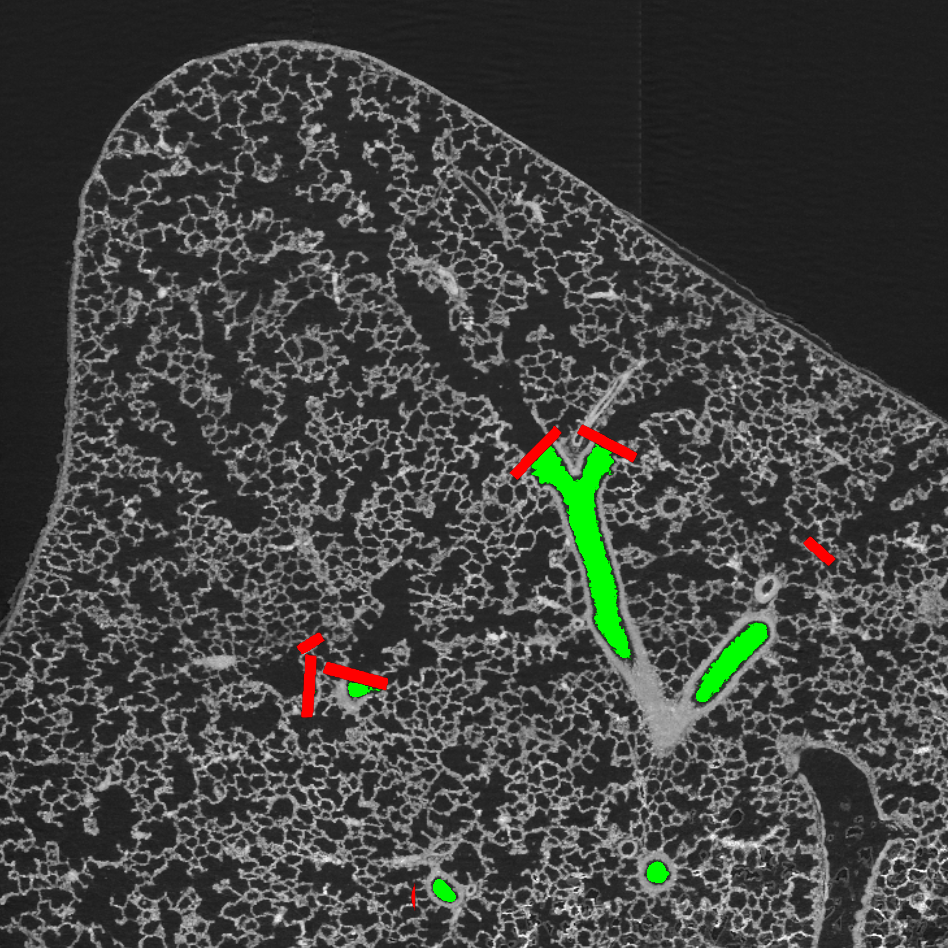
\includegraphics[width=\imagewidth]{img/ManholeCoverExplanation/60B_sagittal_slice_415}};
		% 948px = 1.403mm > 100px = 148um > 338px = 500um, 68px = 100um
		\draw[|-|,white,thick] (\x,\y) -- (\x+338,\y) node [midway,above] {\SI{500}{\micro\meter}};
		\filldraw[yellow,dashed,ultra thick,fill opacity=0.2](508,436) circle (20);
		\filldraw[yellow,dashed,ultra thick,fill opacity=0.2] (617,407) circle (20);
		\filldraw[yellow,dashed,ultra thick,fill opacity=0.2](642,434) circle (20);
		\filldraw[yellow,dashed,ultra thick,fill opacity=0.2](385,663) circle (20);
		\filldraw[yellow,dashed,ultra thick,fill opacity=0.2](347,653) circle (15);
		\filldraw[yellow,dashed,ultra thick,fill opacity=0.2] (245,667) circle (20);
		\node at (537+\s,451+\s) {1};
		\node [white] at (537,451) {1};
		\node at (606+\s,443+\s) {2};
		\node [white] at (606,443) {2};
		\node at (308+\s,683+\s) {3};
		\node [white] at (308,683) {3};
		\node at (353+\s,674+\s) {4};
		\node [white] at (353,674) {4};
		\node at (818+\s,550+\s) {5};
		\node [white] at (818,550) {5};
		\node at (309+\s,643+\s) {6};
		\node [white] at (309,643) {6};
	\end{tikzpicture}%
	\caption{Sagittal slice of one tomographic dataset showing extracted conducting airways in green and several manhole covers in red.
		The dashed yellow circles highlight some examples of alveoli which mark the change from conducting to gas-exchanging regions.
		Changes in thickness and structure of the epithelium and of the wall itself were also used to identify the entrances of the acini.
		Four manhole covers are shown cut right through the middle (\numrange{1}{4}), two manhole covers are only partially cut in this slice and thus appear much smaller (5 \& 6).}
	\label{fig:ManholeCoverExplanation}
\end{figure}

Once all acinar entrance points were defined, we extracted the volume of each isolated acinus (shown as yellow volumes in \autoref{subfig:extracted acini}) in an automated third step.
The manhole covers were defined by their diameter and \href{https://secure.wikimedia.org/wikipedia/en/w/index.php?title=Surface_normal&oldid=411684319}{surface normal}.
We extracted the volume of the single acini using an additional region growing module.
A point along the surface normal defining the manhole cover was used as seed point for this region growing segmentation.
The only manual work needed for the final extraction of the volume of each acinus was the iterative selection of the appropriate segmentation threshold and subsequent tabulation of the automatically calculated acinar volume.

\renewcommand{\imsize}{0.33\linewidth}%
\pgfmathsetlength{\imagewidth}{\imsize}%
\pgfmathsetlength{\imagescale}{\imagewidth/800}%
\def\x{55}
\def\y{745}
\begin{figure}
	\centering
	\subfloat[Sample]{%
		\begin{tikzpicture}[x=\imagescale,y=-\imagescale]
			\node[anchor=north west, inner sep=0pt, outer sep=0pt] at (0,0) {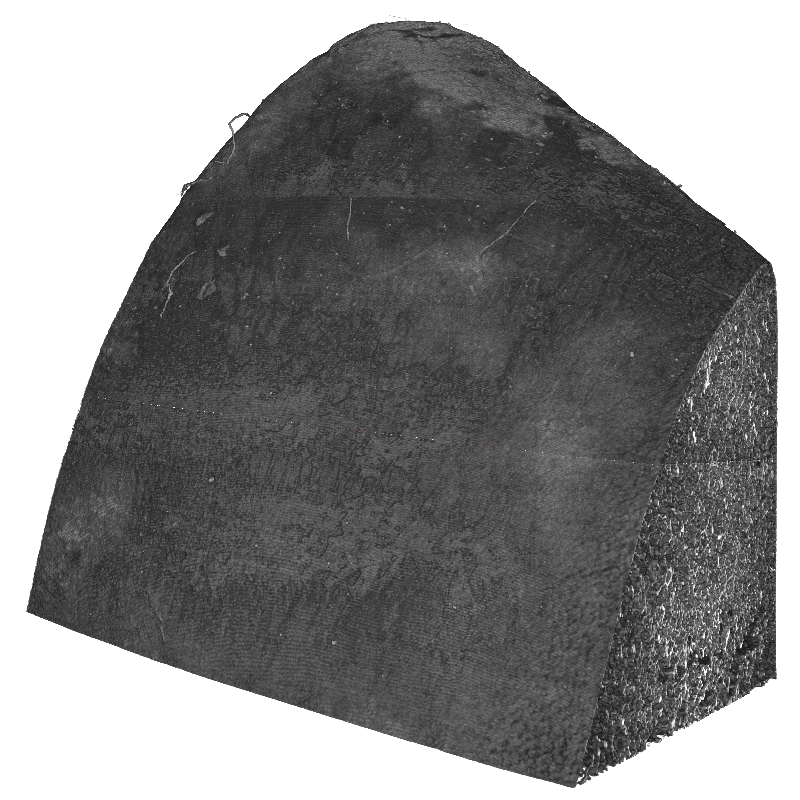
\includegraphics[width=\imagewidth]{img/ManholeCover/R108C60B_2010c_Sample}};
			% 570px = 4.363mm > 100px = 765um > 65px = 500um, 13px = 100um
			%\draw[|-|,blue,thick] (30,608) -- (571,788) node [sloped,midway,above,fill=white,semitransparent,text opacity=1] {\SI{4.363}{\milli\meter} (2948px) TEMPORARY!};
			\draw[|-|,thick] (\x,\y) -- (\x+65,\y) node [right] {\SI{500}{\micro\meter}};
			\draw[dashed,green,thick] (777,460) -- (662,466) -- (84,394);
			\draw[dashed,green,thick] (723,223) -- (181,201);
		\end{tikzpicture}%
		\label{subfig:sample}%
		}%
	\subfloat[Extracted conducting airways with manhole covers shown overlaid over Sample.]{%
		\begin{tikzpicture}[x=\imagescale,y=-\imagescale]
			\node[anchor=north west, inner sep=0pt, outer sep=0pt] at (0,0) {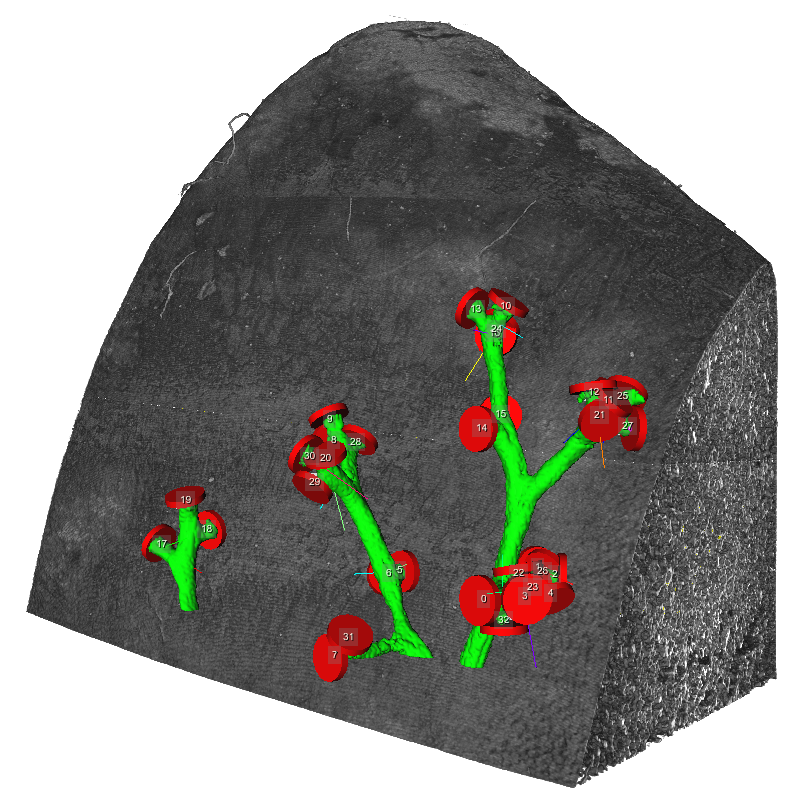
\includegraphics[width=\imagewidth]{img/ManholeCover/R108C60B_2010c_Sample_Airway}};
			% 570px = 4.363mm > 100px = 765um > 65px = 500um, 13px = 100um
			%\draw[|-|,thick] (\x,\y) -- (\x+65,\y) node [right] {\SI{500}{\micro\meter}};
		\end{tikzpicture}%
		\label{subfig:airway segment}%
		}%
	\subfloat[Extracted acini.]{%
		\begin{tikzpicture}[x=\imagescale,y=-\imagescale]
			\node[anchor=north west, inner sep=0pt, outer sep=0pt] at (0,0) {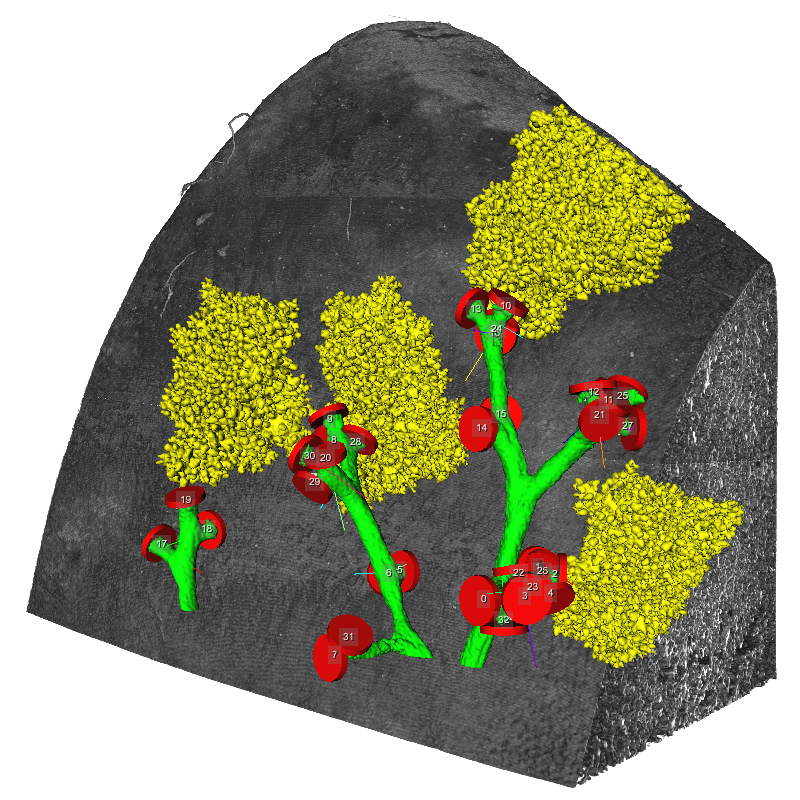
\includegraphics[width=\imagewidth]{img/ManholeCover/R108C60B_2010c_Sample_Acini}};
			%\draw[|-|,thick] (\x,\y) -- (\x+65,\y) node [right] {\SI{500}{\micro\meter}};
		\end{tikzpicture}%
		\label{subfig:extracted acini}%
		}%
	\caption{%
		Visualization of the work flow for the extraction of the acinar volumes in a rat lung sample (postnatal day 60): %
		\protect\subref{subfig:sample}: Three-dimensional visualization of the sample.
		To increase the field of view  a stack of three wide field scans were taken.
		The borders between the three stacked scans are indicated by a dashed green line. 
		\protect\subref{subfig:airway segment} Extracted airway segment (green) superimposed on the sample.
		Using a grey-level threshold based region growing algorithm , we extracted conducting airways inside the sample.
		The red discs (nicknamed manhole covers) were semiautomatically placed and used as segmentation stoppers for the region growing during segmentation of individual acini.
		\protect\subref{subfig:extracted acini} Four extracted acini are shown superimposed over the sample in yellow.
	}
	\label{fig:workflow}
\end{figure}

The volume of the single acini was calculated by multiplying the amount of segmented voxels by the voxel volume.
The single acini were exported to \href{https://secure.wikimedia.org/wikipedia/en/w/index.php?title=Digital_Imaging_and_Communications_in_Medicine&oldid=415023605}{DICOM} files for further processing as described below.
The exported files contained a combination of the segmented acinar volume in the foreground with the corresponding region of interest of the original tomographic dataset in the background, as seen in \autoref{fig:STEPanizer David}.

\subsection{Stereological Analysis}
To check the calculated volumes against a gold standard method, we stereologically estimated the volume of the individual acini.
To guarantee accurate and unbiased results, we standardized each step of tissue fixation, processing sampling and analysis and performed the stereological estimation according to \citet{Hsia2010}.

A MATLAB\textsuperscript{\textregistered} script was used to perform a systematic random sampling of slices of each individual acinus and to export the selected slices as JPG sequences for stereological analysis.

Using the web-based stereology freeware STEPanizer~\cite[\url{http://stepanizer.com}]{Tschanz2011} we analyzed the volume, surface area and number of alveoli of the extracted acini.
Intersections of the acinar surface with geometric line probes were counted to estimate the acinar surface, while simple point counting was used to estimate the volume of the extracted acini.
Alveolar number was estimated by counting the number of entrance rings in paired sections by using the disector mode of the STEPanizer \cite{Hsia2010} (\autoref{fig:STEPanizer David} and \ref{fig:STEPanizer Evelyne}).

\renewcommand{\imsize}{\linewidth}%
\pgfmathsetlength{\imagewidth}{\imsize}%
\pgfmathsetlength{\imagescale}{\imagewidth/1280}%
\begin{figure}
	\centering
	\begin{tikzpicture}[x=\imagescale,y=-\imagescale]
		\node[anchor=north west, inner sep=0pt, outer sep=0pt] at (0,0) {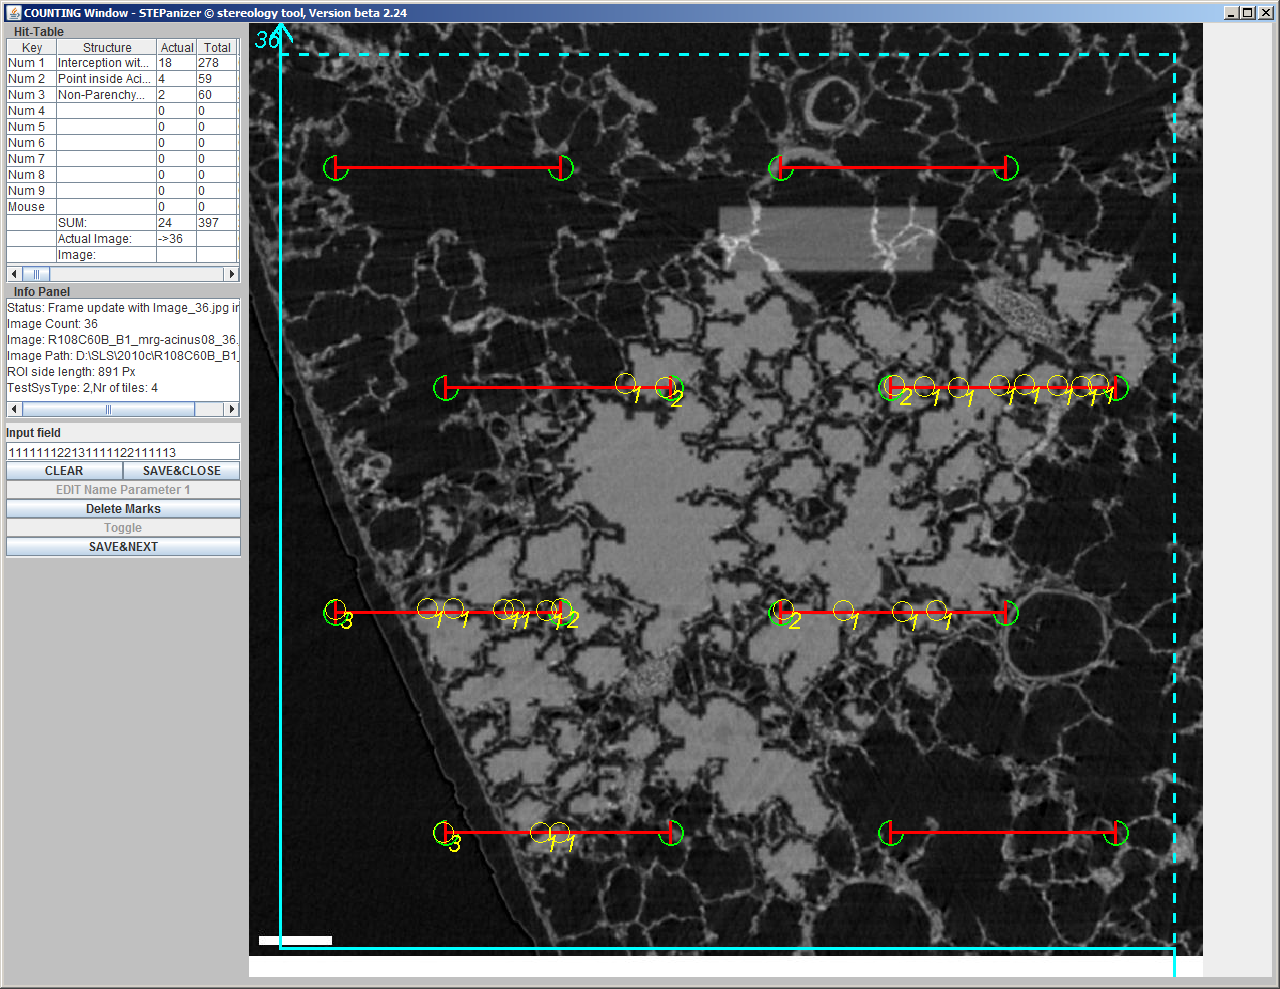
\includegraphics[width=\imagewidth]{img/STEPanizer_2010_R108C60B_acinus08_Slice36}};
		% 914px = 0.1mm > 100px = 11um > 4568px = 500um, 914px = 100um
		\draw[dashed,green,thick] (719,207) -- (937,207) -- (932,270) -- (723,270) -- cycle ;
	\end{tikzpicture}%
	\caption{Screenshot from the STEPanizer counting window.
		The segmented acinus is visible in light grey, the manhole cover which was used to separate this acinus is visualized with a dashed green line for display purposes.
		Both structures have been merged with the original tomographic data using the described MeVisLab work flow and exported to single JPG files.
		Line and point probes used for counting are shown as red lines and green circles.
		Scale bar: \SI{100}{\micro\meter}.}
	\label{fig:STEPanizer David}
\end{figure}

\renewcommand{\imsize}{0.5\linewidth}
\begin{figure}
	\centering
	\subfloat[Disector mode, Image a]{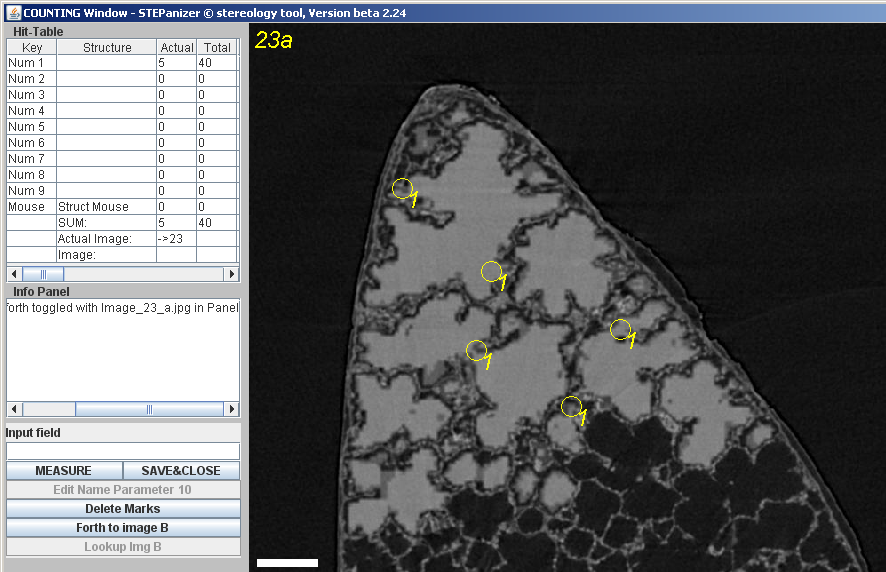
\includegraphics[width=\imsize]{img/R108C60B_B1_mrg-acinus10_EntranceCountingA_crop_edit}}
	\subfloat[Disector mode, Image b]{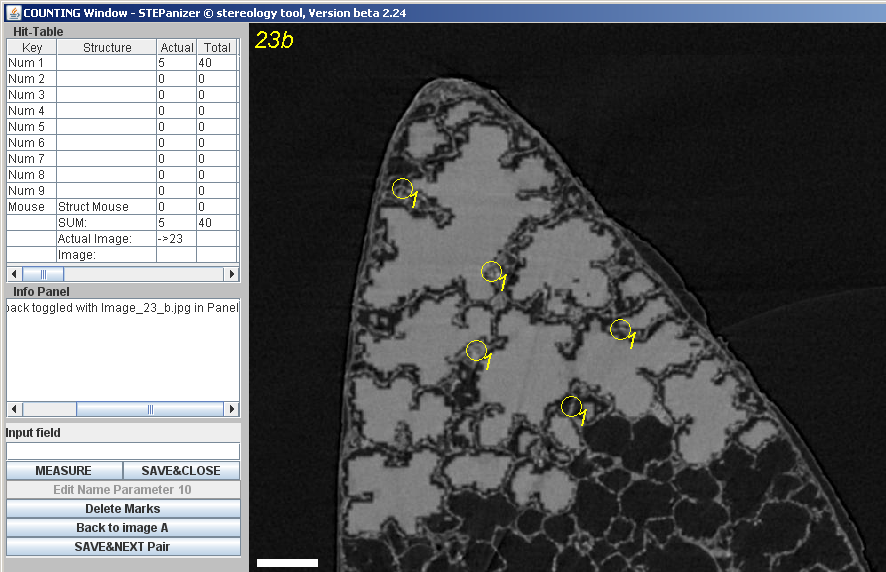
\includegraphics[width=\imsize]{img/R108C60B_B1_mrg-acinus10_EntranceCountingB_crop_edit}}
	\caption{Cropped screenshots from the STEPanizer counting window in disector mode.
		The segmented acinus is visible in light grey, appearing and disappearing bridges corresponding to alveolar entrance rings are counted and marked by yellow circles.
		Scale bar: \SI{100}{\micro\meter}.}
	\label{fig:STEPanizer Evelyne}
\end{figure}

\section{Results}
\label{sec:results}
\subsection{Segmentation of acini}
The novel method described in \autoref{sec:manhole covers} was used to extract individual functional units of three rat lungs from high resolution synchrotron radiation based tomographic datasets.
Using a simple visual approach to mark changes in the airway wall structure (\autoref{fig:ManholeCoverExplanation}) we pinpointed the locations of  so-called manhole covers.
These manhole covers acted as segmentation stoppers, enabled an automated closing of the airways tree and the following grey-level threshold based region growing segmentation permitted us to efficiently extract \numberofacini\xspace acini for stereological analysis.
To our best knowledge, such an extraction of rat lung acini from large high resolution tomographic datasets has never been achieved before and enables us to provide data on acinar volume, surface area and numbers of alveoli per acinus.

\subsection{Acinar volume}
The volume of individual acini was either automatically assessed by adding the segmented voxels inside the acini and multiplying them with the voxel volume or manually estimated by using the Cavaglieri method~\citep{Hsia2010} using the STEPanizer.
Their mean volume is \SI{\meanacinarvolume}{\centi\metre\cubed}, with a standard deviation of \SI{\std}{\centi\metre\cubed}. We removed \numberofoutliers\xspace outliers from the volume data because their value was larger than the mean volume value \(\pm\biggerthan\times\) standard deviations (red dots in \autoref{fig:Volume plots}).

\renewcommand{\imsize}{0.33\linewidth}
\begin{figure}
	\centering
	\subfloat[Acinus 10, location in sample]{%
		\pgfmathsetlength{\imagewidth}{\imsize}%
		\pgfmathsetlength{\imagescale}{\imagewidth/701}%
		\def\x{55}% scalebar-x at golden ratio of x=701px
		\def\y{721}% scalebar-y at 90% of height of y=801px
		%%\begin{minipage}[c][1\width]{\imsize}%
			\begin{tikzpicture}[x=\imagescale,y=-\imagescale]
				\clip (0,0) rectangle (701,801);
				\node[anchor=north west, inner sep=0pt, outer sep=0pt] at (0,0) {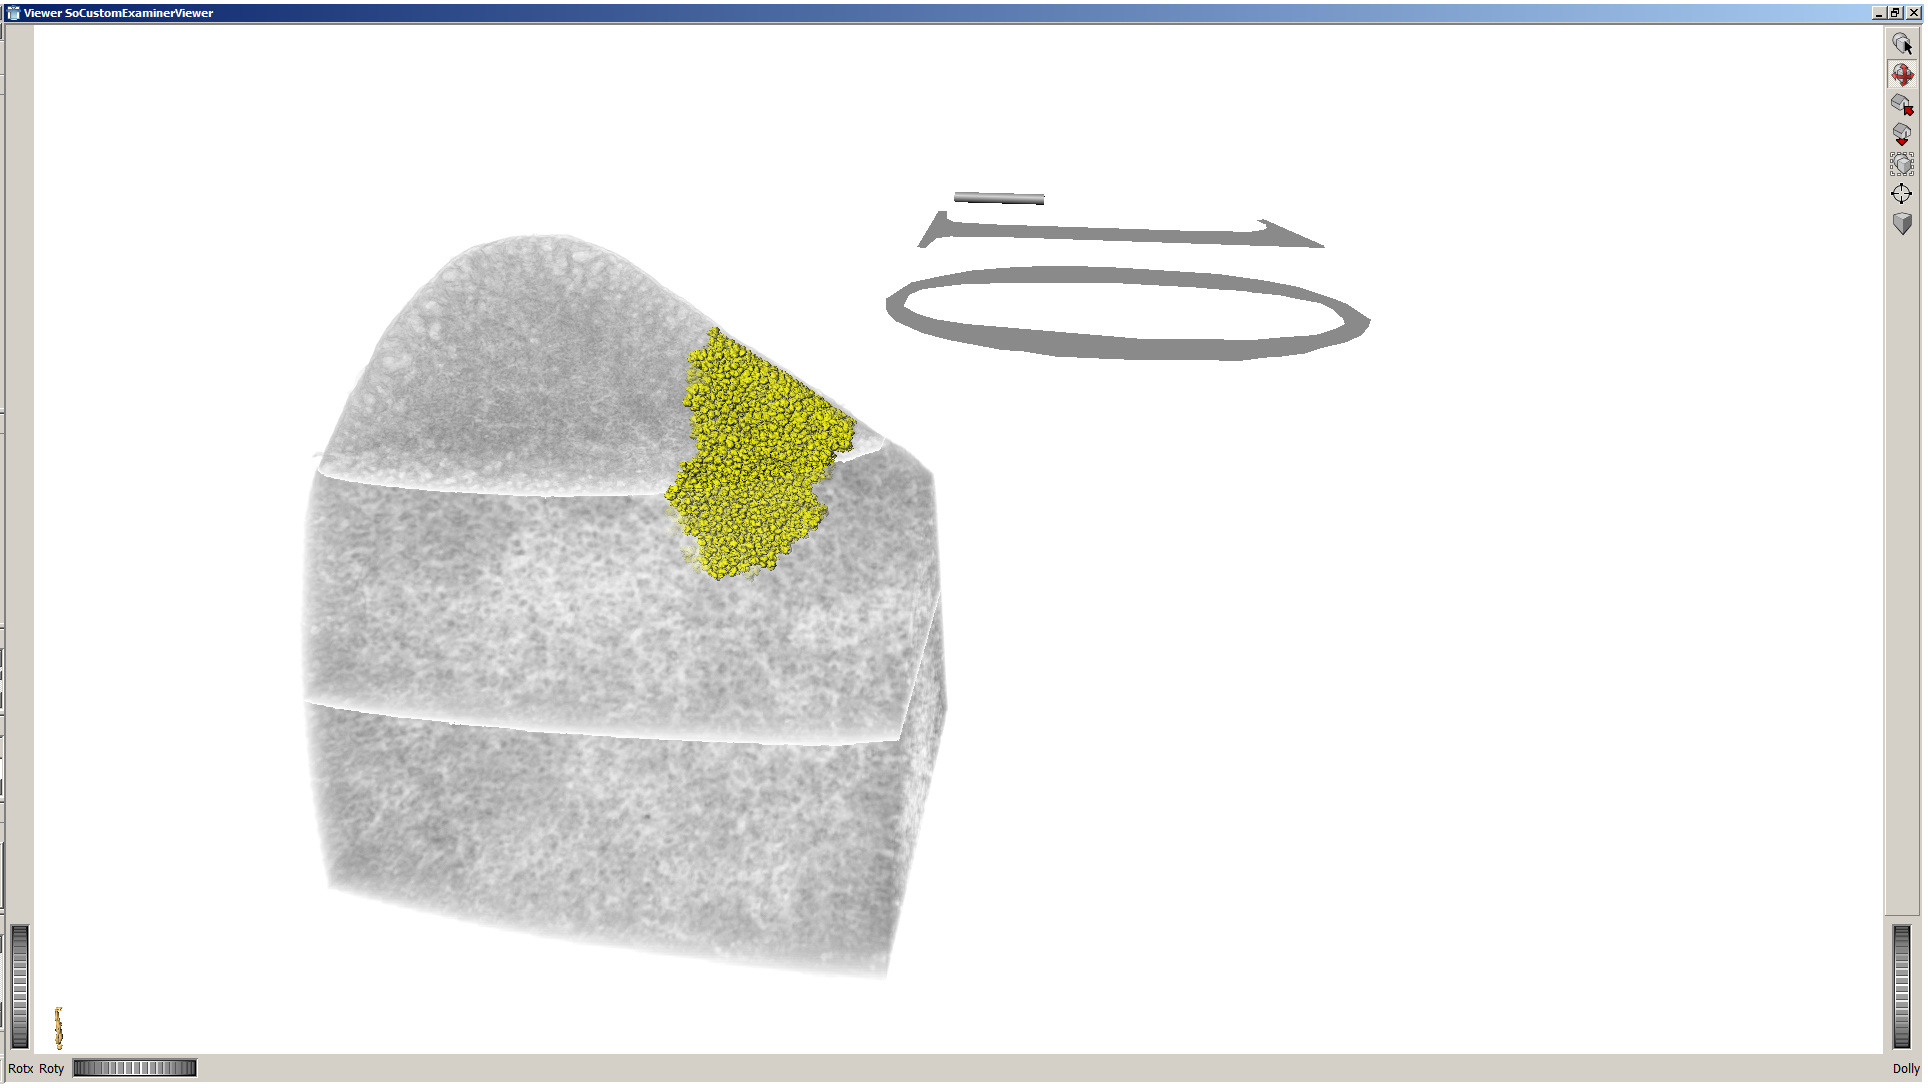
\includegraphics[width=\imagewidth]{img/SingleAcinusFullView/acinus10_01}};
				\draw[|-|,thick] (\x,\y) -- (\x+65,\y) node [right] {\SI{500}{\micro\meter}};
\end{tikzpicture}%
		%%\end{minipage}
		}%
	\subfloat[Acinus 10, view 1]{%
		\pgfmathsetlength{\imagewidth}{\imsize}%
		\pgfmathsetlength{\imagescale}{\imagewidth/718}%
		%\begin{minipage}[c][1\width]{\imsize}%
			\begin{tikzpicture}[x=\imagescale,y=-\imagescale]
				\clip (0,0) rectangle (718,576);
				\node[anchor=north west, inner sep=0pt, outer sep=0pt] at (0,0) {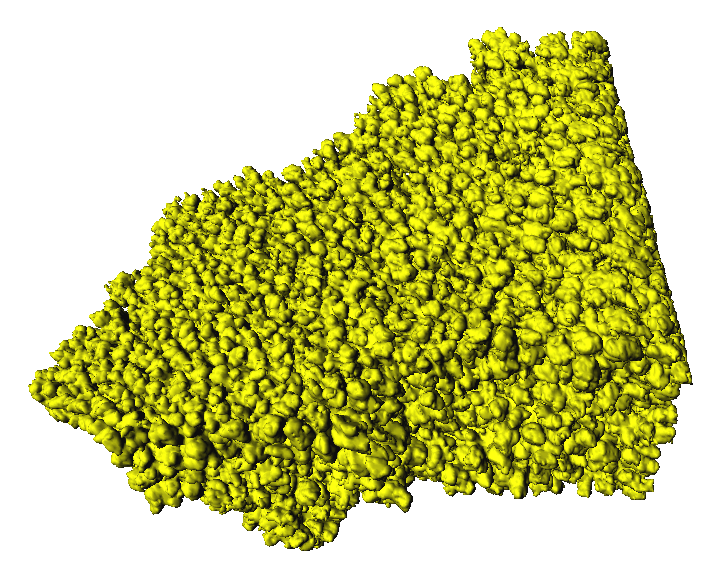
\includegraphics[width=\imagewidth]{img/SingleAcinusFullView/acinus10_03}};
				\draw[red,semitransparent, ultra thick, rotate around={-5:(340,428)}] (340,428) ellipse (70 and 20);
			\end{tikzpicture}%
		%\end{minipage}
		}%
	\subfloat[Acinus 10, view 2]{%
		\pgfmathsetlength{\imagewidth}{\imsize}%
		\pgfmathsetlength{\imagescale}{\imagewidth/1169}%
		%\begin{minipage}[c][1\width]{\imsize}%
			\begin{tikzpicture}[x=\imagescale,y=-\imagescale]
				\clip (0,0) rectangle (1169,959);
				\node[anchor=north west, inner sep=0pt, outer sep=0pt] at (0,0) {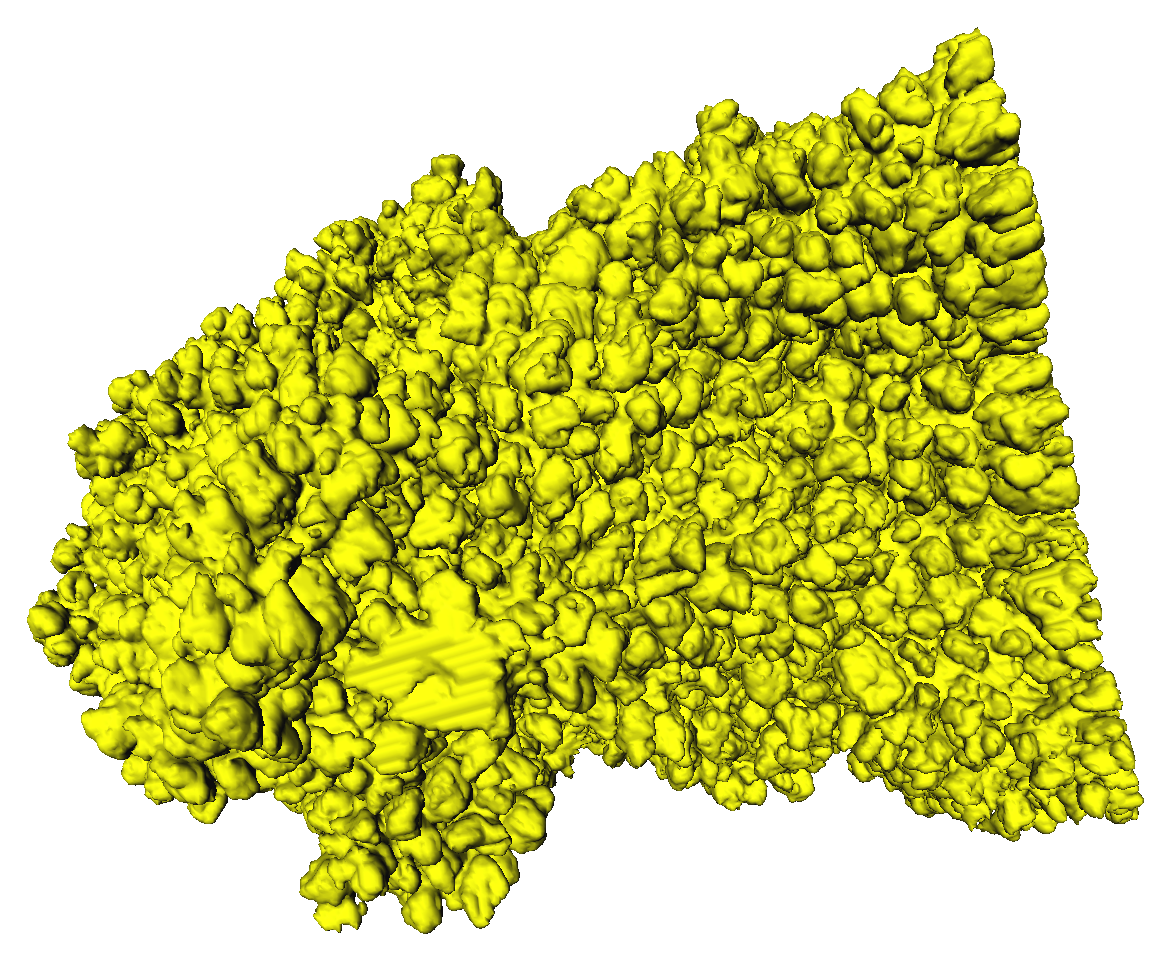
\includegraphics[width=\imagewidth]{img/SingleAcinusFullView/acinus10_04}};
				\draw[red,semitransparent, ultra thick] (422,647) ellipse (115 and 80);
			\end{tikzpicture}%
		%\end{minipage}
		}%
	\\%
	\subfloat[Acinus 26, location in sample]{%
		\pgfmathsetlength{\imagewidth}{\imsize}%
		\pgfmathsetlength{\imagescale}{\imagewidth/833}%
		\def\x{55}% scalebar-x at golden ratio of x=833px
		\def\y{756}% scalebar-y at 90% of height of y=840px
		%\begin{minipage}[c][1\width]{\imsize}%
			\begin{tikzpicture}[x=\imagescale,y=-\imagescale]
				\clip (0,0) rectangle (833,840);
				\node[anchor=north west, inner sep=0pt, outer sep=0pt] at (0,0) {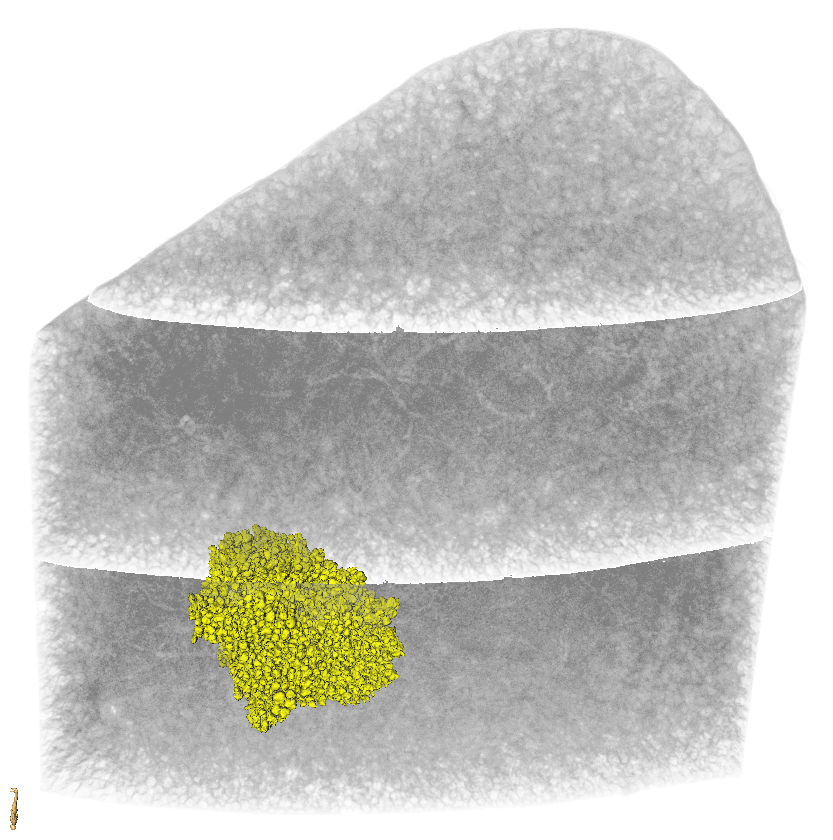
\includegraphics[width=\imagewidth]{img/SingleAcinusFullView/acinus26_07}};
				% 702px = 4.363mm > 100px = 621um > 80px = 500um, 16px = 100um
				%\draw[|-|,blue,thick] (40,791) -- (742,775) node [sloped,midway,above,fill=white,semitransparent,text opacity=1] {\SI{4.363}{\milli\meter} (2948px)};
				\draw[|-|,thick] (\x,\y) -- (\x+80,\y) node [right] {\SI{500}{\micro\meter}};
			\end{tikzpicture}%
		%\end{minipage}
		}%
	\subfloat[Acinus 26, view 1]{%
		\pgfmathsetlength{\imagewidth}{\imsize}%
		\pgfmathsetlength{\imagescale}{\imagewidth/1089}%
		%\begin{minipage}[c][1\width]{\imsize}%
			\begin{tikzpicture}[x=\imagescale,y=-\imagescale]
				\clip (0,0) rectangle (1089,880);
				\node[anchor=north west, inner sep=0pt, outer sep=0pt] at (0,0) {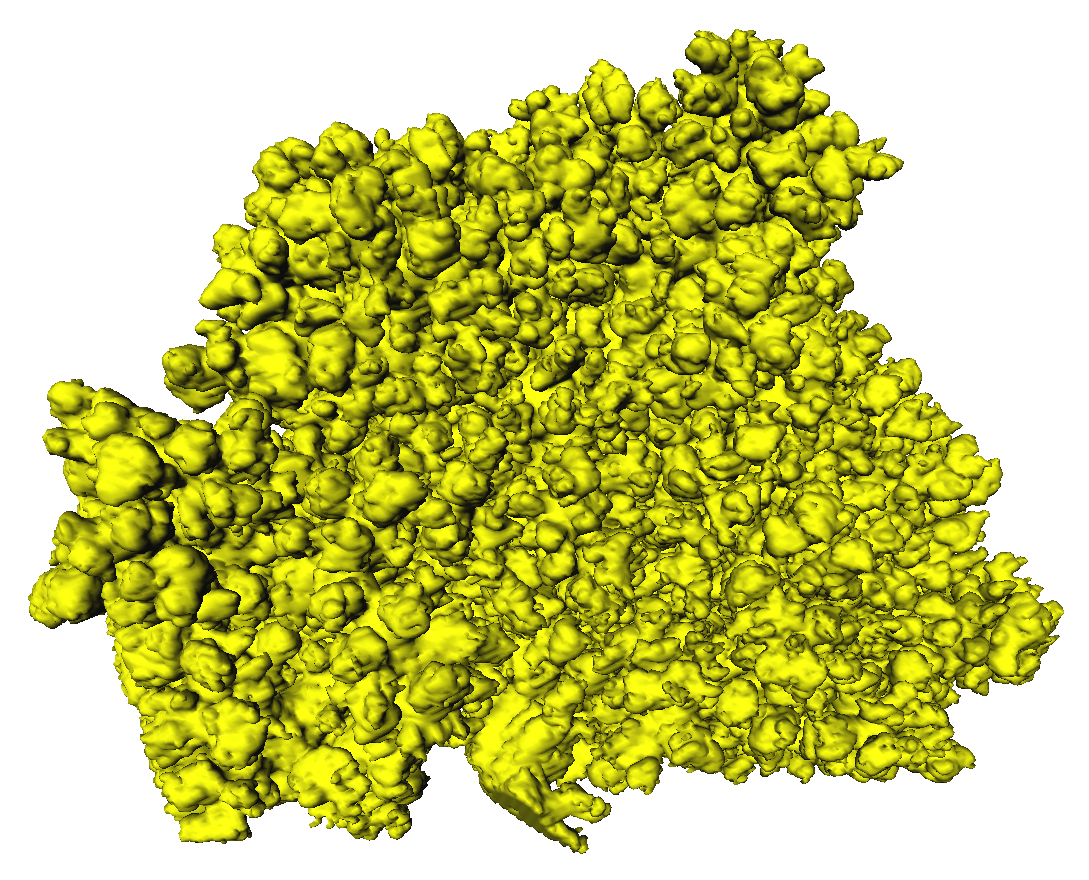
\includegraphics[width=\imagewidth]{img/SingleAcinusFullView/acinus26_11}};
				\draw[red,semitransparent,ultra thick,rotate around={-40:(524,802)}] (524,802) ellipse (70 and 40);
			\end{tikzpicture}%
		%\end{minipage}
		}%
	\subfloat[Acinus 26, view 2]{%
		\pgfmathsetlength{\imagewidth}{\imsize}%
		\pgfmathsetlength{\imagescale}{\imagewidth/839}%
		%\begin{minipage}[c][1\width]{\imsize}%
			\begin{tikzpicture}[x=\imagescale,y=-\imagescale]
				\clip (0,0) rectangle (830,953);
				\node[anchor=north west, inner sep=0pt, outer sep=0pt] at (0,0) {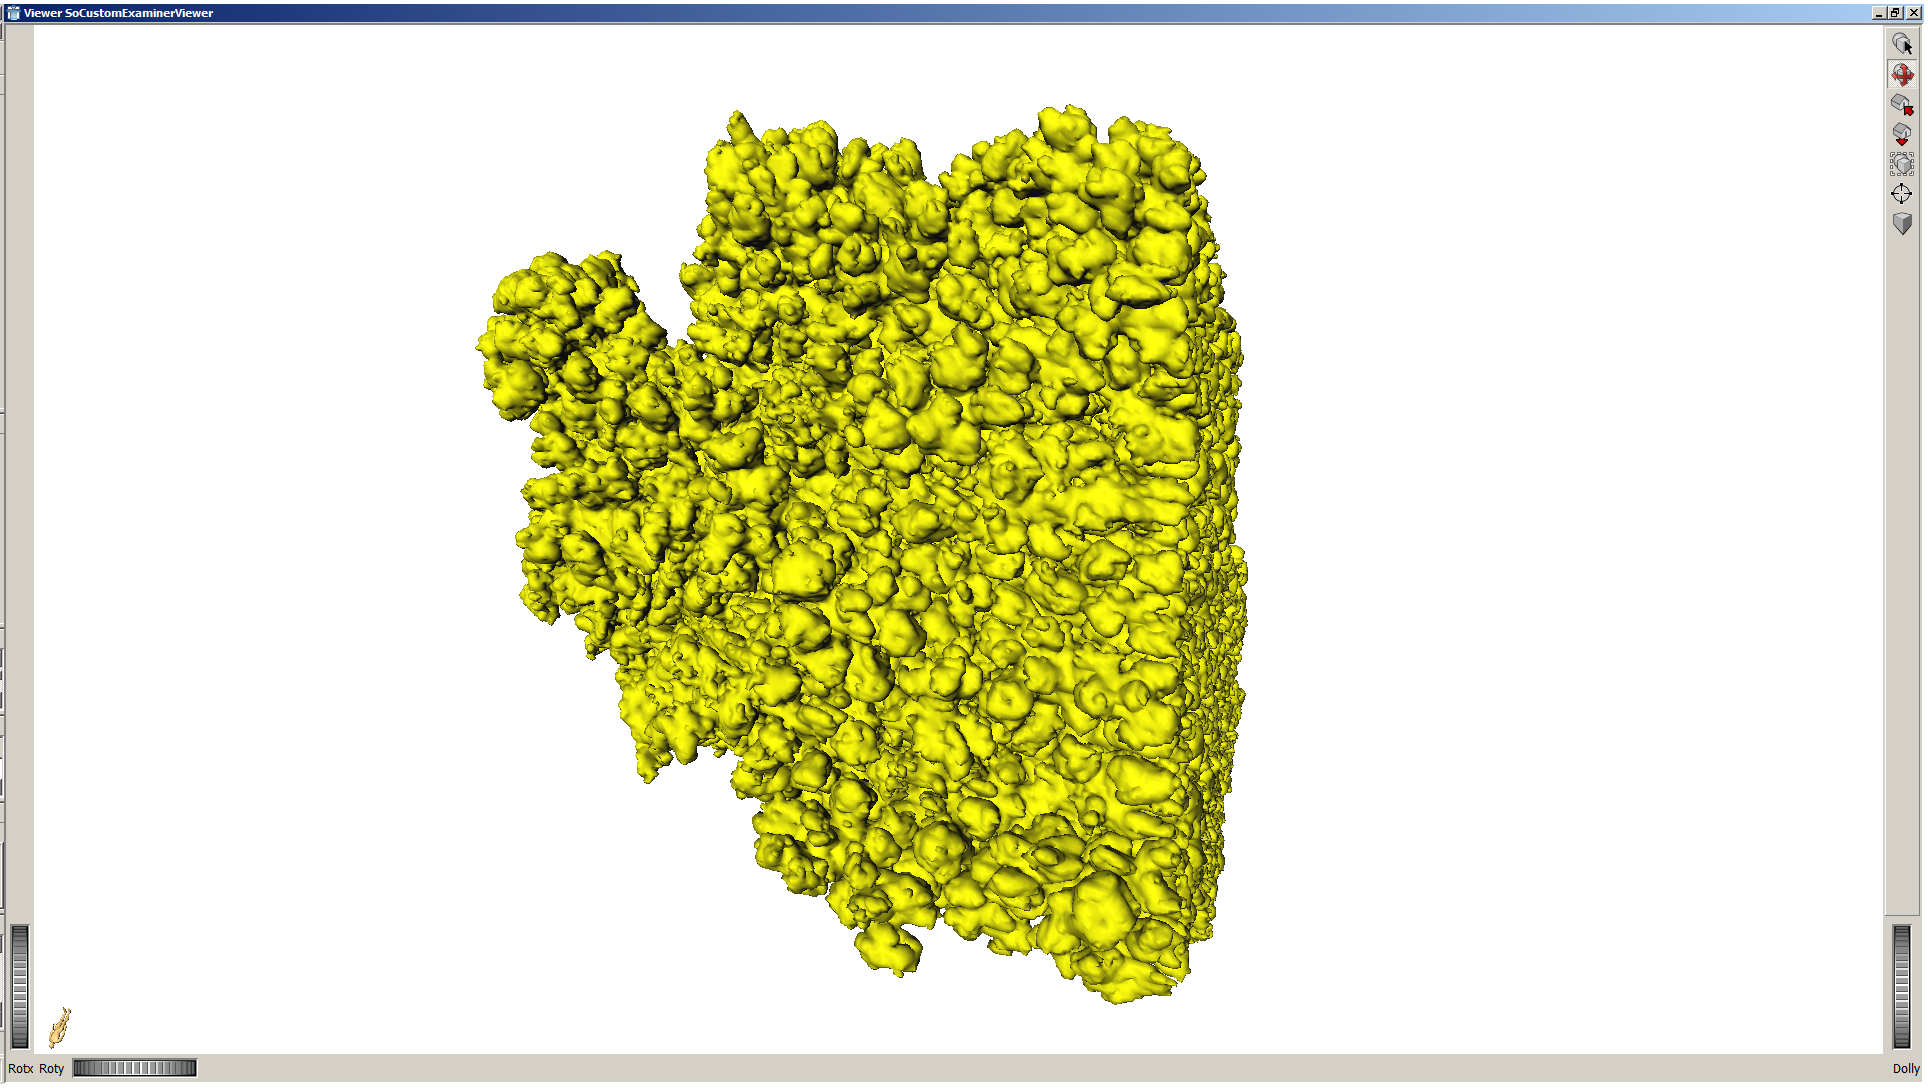
\includegraphics[width=\imagewidth]{img/SingleAcinusFullView/acinus26_13}};
			\end{tikzpicture}%
		%\end{minipage}
		}%
	\caption{Views of two sample acini from rat 1. Left: Location in the sample, Middle: View 1, Right: View 2. The inset mannequin on the lower right shows the three-dimensional orientation, the semitransparent circles mark the approximate position of the manhole cover, whenever visible.}
	\label{fig:acini}
\end{figure}

\subsection{Acinar surface area}
To automatically extract the surface of the single acini a three-dimensional triangulation of the surface would be needed, \ie the extent of the voxels has to be mapped to adjoining triangles in the three-dimensional space.
Since the triangulation of the surface inherently poses a classic Coast of Wales-problem~\citep{Mandelbrot1967a} and is heavily depending on the resolution of the used dataset, we did not automatically calculate the surface (\eg using MeVisLab), but stereologically estimated the surface of the acini by counting interception of test lines with the acinar septa~\citep{Hsia2010}.
Because we assessed our datasets at their original resolution (equal to a light microscope operating with a 10x objective lens), the Coast of Wales-problem was only dependent on the original resolution and not on the need of binning our datasets due to limitation of the computing power. 

For the three different animals we calculated a mean acinar surface of \SI{\meanacinarsurface}{\centi\metre\squared} (%
animal 1: \SI{\acinarsurfaceB}{\centi\metre\squared},
animal 2: \SI{\acinarsurfaceD}{\centi\metre\squared} and
animal 3: \SI{\acinarsurfaceE}{\centi\metre\squared}).

%With the number of acini calculated above, this translates to a mean airspace surface of \SI{\meanairspacesurface}{\centi\metre\squared} (%
%animal 1: \SI{\airspacesurfaceB}{\centi\metre\squared},
%animal 2: \SI{\airspacesurfaceD}{\centi\metre\squared} and
%animal 3: \SI{\airspacesurfaceE}{\centi\metre\squared}).

\subsection{Number of alveoli per acinus}
By counting appearing and disappearing bridges in the segmented acini, we found a mean number of alveoli for all analyzed acini of \meannumberofalveoli\xspace (%
individual mean for animal 1: \numberofalveoliB\xspace (\numberofaciniB\xspace acini analyzed),
individual mean for animal 2: \numberofalveoliD\xspace (\numberofaciniD\xspace acini analyzed),
individual mean for animal 3: \numberofalveoliE\xspace (\numberofaciniE\xspace acini analyzed)).

\subsection{Total number of acini}
We estimated an absolute number of acini per lung by dividing the absolute parenchymal volume by the mean acinar volume.
For the three lung investigated we calculated \totalnumberofaciniB, \totalnumberofaciniD\xspace and \totalnumberofaciniE\xspace acini per lung, respectively, resulting in a mean of \meantotalnumberofacini\xspace with a standard deviation of \meantotalnumberofaciniSTD.

The absolute number of acini per lung can also be estimated by dividing the estimated total number of alveoli (personal communication Stefan Tschanz) by the number of alveoli per acinus.
For the three lung investigated we calculated \totalnumberofaciniBVariant, \totalnumberofaciniDVariant\xspace and \totalnumberofaciniEVariant\xspace acini per lung, respectively, resulting in a mean of \meantotalnumberofaciniVariant\xspace with a standard deviation of \meantotalnumberofaciniSTDVariant.

\subsection{Comparison of Volumes from MeVisLab with STEPanizer}\todo{Irgendwie halt doch mehr Resultate als Diskussion, auch mit Plots\ldots}
We compared the automatically assessed and manually estimated volume of the individual acini and found that the manual stereological method results in a \difference\(\times\) larger value than the automatic method using voxel counting.
Detailed results are shown in \autoref{fig:Volume plots} and explained later on in the Discussion section.
Values larger than the mean of the volumes \(\pm\biggerthan\times\) the standard deviation have been removed from the calculation (red dots).

\begin{figure}
	\centering
	\subfloat{
		\begin{tikzpicture}

\begin{axis}[
	width=\imsize,
	xlabel={Acinus},
	ylabel={Volume [\si{\milli\meter\cubed}]},
	ymin=1e-7, ymax=4,
	scaled ticks=true,
	%yticklabel=\empty
	]
\addplot [red, only marks]
coordinates {
(0,0.37731293) (1,0.19965522) (2,0.25447792) (3,0.43383464) (4,nan) (5,0.31837037) (6,0.42459121) (7,nan) (8,0.294278) (9,0.26970762) (10,0.47316542) (11,0.13395399) (12,0.2331105) (13,nan) (14,0.66745716) (15,0.45502964) (16,nan) (17,nan) (18,0.47915584) (19,nan) (20,0.43513966) (21,0.33121431) (22,0.15090302) (23,nan) (24,0.14413643) (25,nan) (26,0.24587891) (27,0.27121842) (28,0.16399051) (29,0.38648456) (30,0.32862523) (31,0.19227928) 
};
\addplot [green, only marks]
coordinates {
(0,0.37731293) (1,0.19965522) (2,0.25447792) (3,0.43383464) (4,nan) (5,0.31837037) (6,0.42459121) (7,nan) (8,0.294278) (9,0.26970762) (10,0.47316542) (11,0.13395399) (12,0.2331105) (13,nan) (14,nan) (15,0.45502964) (16,nan) (17,nan) (18,0.47915584) (19,nan) (20,0.43513966) (21,0.33121431) (22,0.15090302) (23,nan) (24,0.14413643) (25,nan) (26,0.24587891) (27,0.27121842) (28,0.16399051) (29,0.38648456) (30,0.32862523) (31,0.19227928) 
};
\addplot [cyan]
	coordinates {
		(0,0.304196244782609) (32,0.304196244782609)
	};
\addplot [cyan, dashed]
	coordinates {
		(0,0.634325534516513) (32,0.634325534516513) 
	};
\addplot [cyan, dashed]
	coordinates {
		(0,-2.59330449512958e-02) (32,-2.59330449512958e-02) 
	};

\end{axis}

\end{tikzpicture}%
		}\hfill%
	\subfloat{
		\begin{tikzpicture}

\begin{axis}[
	width=\imsize,
	xlabel={Acinus},
	%ylabel={Volume [\si{\centi\meter\cubed}]},
	ymin=1e-7, ymax=4,
	]
\addplot [red, only marks]
coordinates {
(0,nan) (1,nan) (2,nan) (3,0.5900293) (4,0.55371433) (5,nan) (6,nan) (7,0.29986489) (8,nan) (9,0.39014131) (10,0.29307008) (11,nan) (12,nan) (13,nan) (14,nan) (15,0.42841768) (16,nan) (17,nan) (18,0.4532719) (19,0.23229824) (20,nan) (21,nan) (22,nan) (23,0.58026904) (24,nan) (25,nan) (26,0.51905155)
};
\addplot [green, only marks]
coordinates {
(0,nan) (1,nan) (2,nan) (3,0.5900293) (4,0.55371433) (5,nan) (6,nan) (7,0.29986489) (8,nan) (9,0.39014131) (10,0.29307008) (11,nan) (12,nan) (13,nan) (14,nan) (15,0.42841768) (16,nan) (17,nan) (18,0.4532719) (19,0.23229824) (20,nan) (21,nan) (22,nan) (23,0.58026904) (24,nan) (25,nan) (26,0.51905155)
};
\addplot [cyan]
	coordinates {
		(0,0.434012832) (27,0.434012832) 
	};
\addplot [cyan, dashed]
	coordinates {
		(0,0.79918601656343) (27,0.79918601656343) 
	};
\addplot [cyan, dashed]
	coordinates {
		(0,6.88396474365702e-02) (27,6.88396474365702e-02) 
	};

\end{axis}

\end{tikzpicture}
		}\hfill%
	\subfloat{
		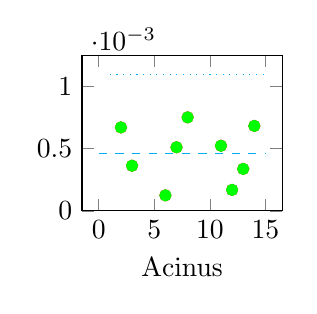
\begin{tikzpicture}

\begin{axis}[
	width=0.34*\linewidth,
	xlabel={Acinus},
	%ylabel={Volume [\si{\centi\meter\cubed}]},
	ymin=1e-7, ymax=1.25e-3,
	]
\addplot [red, only marks]
coordinates {
(0,nan) (1,nan) (2,0.0006709888) (3,0.00036325091) (4,nan) (5,nan) (6,0.00012486846) (7,0.00051163185) (8,0.00075202513) (9,nan) (10,nan) (11,0.00052375108) (12,0.00016866906) (13,0.00033741882) (14,0.00068318522)
};
\addplot [green, only marks]
coordinates {
(0,nan) (1,nan) (2,0.0006709888) (3,0.00036325091) (4,nan) (5,nan) (6,0.00012486846) (7,0.00051163185) (8,0.00075202513) (9,nan) (10,nan) (11,0.00052375108) (12,0.00016866906) (13,0.00033741882) (14,0.00068318522)
};
\addplot [cyan, dashed]
	coordinates {
		(0,0.000459532147777778) (15,0.000459532147777778) 
	};
\addplot [cyan, dotted]
	coordinates {
		(1,0.00109820895859664) (15,0.00109820895859664) 
	};
\addplot [cyan, dotted]
	coordinates {
		(1,-0.000179144663041085) (15,-0.000179144663041085) 
	};

\end{axis}

\end{tikzpicture}
		}\\%
	\subfloat{
		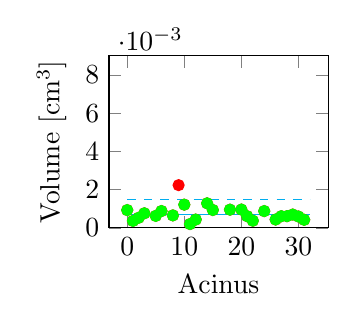
\begin{tikzpicture}

\begin{axis}[
	width=0.36*\linewidth,
	xlabel={Acinus},
	ylabel={Volume [\si{\centi\meter\cubed}]},
	ymin=1e-7, ymax=0.009,
	%ymin=0, ymax=0.0042,
	%yticklabel=\empty
	]
\addplot [red, only marks]
coordinates {
(0,0.000928503038942363) (1,0.000363236072194969) (2,0.000528476198612276) (3,0.000761414474783716) (4,nan) (5,0.000626766920809997) (6,0.000878359350940617) (7,nan) (8,0.000651206767483189) (9,0.00223488663353551) (10,0.00121456308634507) (11,0.000199220648894286) (12,0.000433235998567998) (13,nan) (14,0.00128366813580556) (15,0.00093334944120013) (16,nan) (17,nan) (18,0.000951931319014455) (19,nan) (20,0.000957101812399371) (21,0.000611808517484639) (22,0.000373053974075999) (23,nan) (24,0.000876431577102944) (25,nan) (26,0.000435061652353202) (27,0.000608824085692031) (28,0.000611808517484639) (29,0.000695108832432261) (30,0.000592133625582743) (31,0.000420831138489319) 
};
\addplot [green, only marks]
coordinates {
(0,0.000928503038942363) (1,0.000363236072194969) (2,0.000528476198612276) (3,0.000761414474783716) (4,nan) (5,0.000626766920809997) (6,0.000878359350940617) (7,nan) (8,0.000651206767483189) (9,nan) (10,0.00121456308634507) (11,0.000199220648894286) (12,0.000433235998567998) (13,nan) (14,0.00128366813580556) (15,0.00093334944120013) (16,nan) (17,nan) (18,0.000951931319014455) (19,nan) (20,0.000957101812399371) (21,0.000611808517484639) (22,0.000373053974075999) (23,nan) (24,0.000876431577102944) (25,nan) (26,0.000435061652353202) (27,0.000608824085692031) (28,0.000611808517484639) (29,0.000695108832432261) (30,0.000592133625582743) (31,0.000420831138489319) 
};
\addplot [cyan]
	coordinates {
		(0,0.000692873703769207) (32,0.000692873703769207) 
	};
\addplot [cyan, dashed]
	coordinates {
		(0,0.0015013239011447) (32,0.0015013239011447) 
	};
\addplot [cyan, dashed]
	coordinates {
		(0,-0.000115576493606282) (32,-0.000115576493606282) 
	};

\end{axis}

\end{tikzpicture}
		}\hfill%
	\subfloat{
		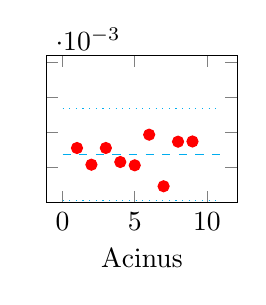
\begin{tikzpicture}

\begin{axis}[
	width=0.33*\linewidth,
	xlabel={Acinus},
	%ylabel={Volume [\si{\centi\meter\cubed}]},
	ymin=0, ymax=0.0042,
	yticklabel=\empty
	]
\addplot [red,only marks]
	coordinates {
		(1,0.00155172120433958)
		(2,0.00107560449835204)
		(3,0.00155219458912006)
		(4,0.00115221850801792)
		(5,0.0010581421745156)
		(6,0.00193194271026777)
		(7,0.000460166958864983)
		(8,0.00173206190419837)
		(9,0.0017382061817182)
	};
\addplot [cyan, dashed]
	coordinates {
		(0,0.00136136208104384) (11,0.00136136208104384) 
	};
\addplot [cyan, dotted]
	coordinates {
		(0,0.00266793742202647) (11,0.00266793742202647) 
	};
\addplot [cyan, dotted]
	coordinates {
		(0,5.47867400612025e-05) (11,5.47867400612025e-05) 
	};
\end{axis}

\end{tikzpicture}
		}\hfill%
	\subfloat{
		\begin{tikzpicture}

\begin{axis}[
	width=\imsize,
	xlabel={Acinus},
	%ylabel={Volume [\si{\centi\meter\cubed}]},
	ymin=1e-7, ymax=4,
	%yticklabel=\empty
	]
\addplot [red, only marks]
coordinates {
(0,nan) (1,nan) (2,1.80894828376899) (3,1.08657864429912) (4,nan) (5,nan) (6,0.213737862253818) (7,2.43389564249541) (8,8.8706408927333) (9,nan) (10,nan) (11,1.90254809872315) (12,0.39743256425486) (13,0.813800299917009) (14,2.45645691813613)
};	
\addplot [green, only marks]
coordinates {
(0,nan) (1,nan) (2,1.80894828376899) (3,1.08657864429912) (4,nan) (5,nan) (6,0.213737862253818) (7,2.43389564249541) (8,nan) (9,nan) (10,nan) (11,1.90254809872315) (12,0.39743256425486) (13,0.813800299917009) (14,2.45645691813613)
};
\addplot [cyan]
	coordinates {
		(0,1.38917478923106) (15,1.38917478923106) 
	};
\addplot [cyan, dashed]
	coordinates {
		(0,3.86715471927792) (15,3.86715471927792) 
	};
\addplot [cyan, dashed]
	coordinates {
		(0,-1.0888051408158) (15,-1.0888051408158) 
	};

\end{axis}

\end{tikzpicture}
		}%
	\caption{Acinar volumes of each sample, extracted with MeVisLab and the STEPanizer. The line corresponds to the mean, the dashed lines correspond to the mean \(\pm\biggerthan\times\) the standard deviation. Red dots are the values removed from the calculation. Top row: MeVisLab volumes, bottom row: STEPanizer volumes. From left to right: animal 1, 2 and 3.}
	\label{fig:Volume plots}
\end{figure}

\begin{table}
	\centering
	\caption{Summary of results}
	\begin{tabular}{rcccc}
	\toprule
															& Animal 1 & Animal 2 & Animal 3 & Mean\\
	\midrule
	Number of analyzed acini 							& \numberofaciniB & \numberofaciniD & \numberofaciniE & \\
	Acinar volume [\si{\cubic\centi\meter}]		& \acinarvolumeB & \acinarvolumeD & \acinarvolumeE & \meanacinarvolume \\
	Acinar surface [\si{\centi\meter\squared}]	& \acinarsurfaceB & \acinarsurfaceD & \acinarsurfaceE & \meanacinarsurface \\
	Total number of acini 								& \totalnumberofaciniB & \totalnumberofaciniD & \totalnumberofaciniE & \meantotalnumberofacini \\
	Alveoli per acinus 									& \numberofalveoliB & \numberofalveoliD & \numberofalveoliE & \meannumberofalveoli \\
	\bottomrule
	\end{tabular}
	\label{tab:results}
\end{table}

\section{Discussion}
The hereby presented method to simply extract single acini from tomographic datasets permits us to estimate parameters like volume, surface area and number of alveoli of single acini, total number of acini and mean airspace surface area in the mammalian lung.

Our proposed method makes it possible to fully analyze biologically interesting parameters of the acini in the lung; the volume of the acini can be extracted automatically, parameters like surface area as well as number of contained alveoli and septal length per acinus (not shown) can be extracted with simple stereological counting, requiring manual labor.

With the proposed method we can additionally analyze structural changes in the acinus during postnatal development, like disease or differences between wild-type and knock-out animals.
All the parameters mentioned above and the structural changes can be obtained for single individual acini, something which is not easily possible using stereological methods on classic tissue sections.

\subsection{Acinar volume}
\citet{Rodriguez1987} found that the right upper lobe of one rat contains 613 acini with a mean volume of \SI{1.98}{\milli\meter\cubed} (\SIrange{0.5}{5}{\milli\meter\cubed}).
\citet{Mercer1987a} state that the total volume of \blockquote{alveoli + ducts} \eg ventilatory units is \SI{0.522(56)}{\cubic\milli\meter} (mean of 8). % http://is.gd/qpMEV5
Our calculations resulted in a volume of \SI{\meanacinarvolume}{\cubic\centi\meter} with a standard deviation of \SI{\std}{\cubic\centi\meter}.
If we take in account that \citep{Mercer1987a} measured the volume of ventilatory units that have been defined half as big as our acinus, then our stereologically estimated mean acinar volume is in the range of previously published data.

\subsection{Acinar surface area}
Missing other published data, we can only relate the estimated surface area to mean values found in literature.
\citet{Tschanz2003} estimated the absolute airspace surface in the rat lung by stereological estimation using electron microscopy images and found a mean absolute airspace surface of \SI{8021}{\centi\metre\squared} for the same animals shown in this study.
By multiplying the number of acini by the mean acinar surface we found the mean absolute airspace surface to be \SI{\meanairspacesurface}{\centi\metre\squared}, a value \airspacedifference\(\times\) smaller.
The differences can be explained largely due to the resolution of the different imaging methods.
For example, \citet{Gehr1978} estimated the alveolar surface area at electron microscopic level and found a \emph{human} alveolar surface area of \SI{143}{\square\meter}, while previous light microscopic estimates \citep{Weibel1963,Thurlbeck1967} found an averaged estimate of the alveolar surface of \SI{82}{\square\meter}, a value 1.744\(\times\) larger, which is also reasoned to be due to the different imaging methods.

\subsection{Number of alveoli per acinus}
\citet{Vasilescu2012} found that the \blockquote{mean number of alveoli per acinus was 596\(\pm\)326 in the young mice and 936\(\pm\)254 in the old mice}. To our best knowledge, the number of alveoli per acinus has never been stereologically estimated for \emph{rat} lungs, making it impossible to relate our result of \meannumberofalveoli\xspace alveoli per acinus to published data.

\subsection{Total number of acini}
We found a mean number of \meantotalnumberofacini\xspace acini per rat lung for our three animals.
\citet{Rodriguez1987} found a total of 4023 acini in the whole lungs for one single rat, while \citet{Mercer1987a} found \blockquote{an estimate of 2020 terminal bronchioles as well as acini per lung}.
\citeauthor{Mercer1987a} mention that differences in these numbers appear to be due the different definition of the acinus, \ie that one ventilatory unit does not correspond to one acinus in their definition.
We did not directly estimate the number of acini, but divided the absolute airspace volume~\citep{Tschanz2003} by the mean acinar volume.
Even though our values are only valid if we assume the acini to possess a similar size throughout the different regions in the lung, our results are comparable to previously published results, showing the feasibility of our method.

\subsection{Comparison of volume estimation methods}
As expected, both methods for volume estimation (MeVisLab vs.\ STEPanizer) show different results; the volumes of single acini estimated with the stereological method show a \difference\(\times\) larger value than when assessed with the automatic method using voxel counting.
Since the automatic calculation of the acinar volume with MeVisLab just adds up all segmented voxels, an imprecise segmentation leads to an underestimation of the acinar volume.
\autoref{fig:MeVisSegmentation} shows exemplary slices for acini with large differences in volume between the two methods.
Due to inevitable segmentation inaccuracies (dark spots inside the segmented acinus in \autoref{subfig:60d_acinus32} we underestimated the volumes with the automatic method compared to the manual, stereological method, where we easily can discard such inaccuracies due the human visual inspection.

In some extracted acini we have seen differences in grey values in the z-direction of the stack.
Since the region growing segmentation method uses the same threshold throughout the region of interest, sometimes single slices were heavily under-estimated in terms of included voxels, one such example is shown in \autoref{subfig:60e_acinus38}.
Since these automatically extracted regions were merely used as an optic guide for the manual, stereological method it is obvious that the manual method shows larger and more precisely estimated volumes than the automatic method, which in contrast is by magnitudes faster.

The underestimation by the automatic method is thus largely due to an incomplete segmentation of the acinar airspace.
As soon as better segmentation methods are becoming available the automated method will become more reliable and accurate.

Manually estimating the volume of the single acini using the STEPanizer took several working days for the few acini shown in \autoref{fig:Volume plots}.
As soon as the manhole covers are defined in the sample, the automatic volume calculation with MeVisLab can be performed in less than a minute per acinus.

\renewcommand{\imsize}{0.56\linewidth}%
\begin{figure}
	\centering
	\hfill%
	%\subfloat[Animal 2, Acinus 32, Slice 45]{%
	\subfloat[Sample acinus from animal 2, Slice 45]{%
		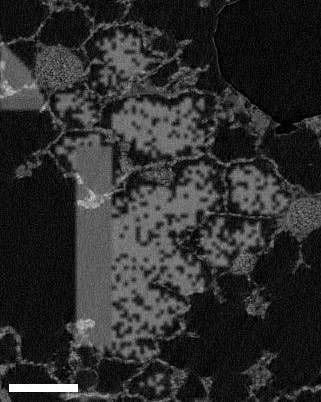
\includegraphics[height=\imsize]{img/Acini/2009f/mrg/R108C60Dt-mrg/acinus32/voxelsize1.48-every6slice/R108C60Dt-mrg-acinus32_45.png}% jpg is unedited!
		\label{subfig:60d_acinus32}%
	}%
	\hfill%
	%\subfloat[Animal 3, Acinus 38, Slice 29]{%
	\subfloat[Sample acinus from animal 3, Slice 29]{%
		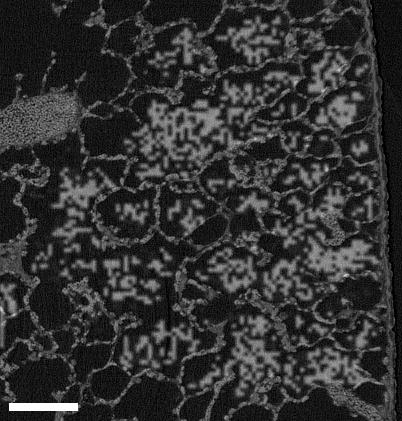
\includegraphics[height=\imsize]{img/Acini/2009f/mrg/R108C60Et-mrg/acinus38/voxelsize1.48-every6slice/R108C60Et-mrg-acinus38_29.png}% jpg is unedited!
		\label{subfig:60e_acinus38}%		
	}%
	\hfill%
	\caption{Illustrative slices of two acini that show large differences in volume between MeVisLab and STEPanizer.
		The inaccurate segmentation is the reason we obtained larger volumes with the STEPanizer than with MeVisLab.
		Panel \protect\subref{subfig:60d_acinus32} shows minor segmentation errors through noise in the paraffin (dark spots inside grey region).
		Panel \protect\subref{subfig:60e_acinus38} shows large segmentation errors.
		Such large errors arise through brightness changes in the dataset which render the threshold chosen for each single acinus unusable for certain slices.
		Scale bar: \SI{100}{\micro\meter}.}
	\label{fig:MeVisSegmentation}
\end{figure}

\section{Conclusions}
The hereby presented manhole cover method is well suited to semiautomatically isolate single acini from three-dimensional datasets for further stereological analysis.
To our knowledge, the presented work flow is the only one published to permit an easy and semiautomatic extraction of single acini.
After the extraction of single acini, a fully automated calculation of the volume of individual acini is possible, thus for the first time enabling the study of large amounts of individual acini in relatively short time.
This opens up the possibility to efficiently estimate biological parameters like volume and surface of single acini, number of acini in the mammalian lung using accepted stereological methods.

We have shown that the achieved results are comparable, differences in results are based on the difference in the counting method and explainable.
Since our proposed method for estimating the volumes of isolated individual acini is by magnitudes faster than manual stereological counting, we believe the presented method is the easiest and fastest way to estimate the volume of very large numbers of single acini in the mammalian lungs.
Unfortunately this is only the case if the threshold based region growing segmentation is very accurate.
If this is not the case \ie if the segmentation is performed with a single threshold, the volume of the individual extracted acini is under-estimated, as shown in \autoref{fig:MeVisSegmentation}.

For this manuscript, the segmentation of the individual acini merely marked the exact region for stereological analysis in the three-dimensional dataset, thus the segmentation and extraction of the individual acini is the prerequisite for the stereological estimation.
This step represents the main amount of time spent evaluating the data, the calculation of the volume of the extracted acini can automatically be performed in a very short time.
With a more advanced segmentation algorithm it would be possible to automatically and accurately estimate the volume of a very large amount of acini, \ie perform a digital Cavalieri estimation of the volume with a point grid of the size of the voxel size of the tomographic data.

\clearpage
\section{Acknowledgments}
We thank Federica Marone, Christoph Hintermüller and Bernd Pinzer for their committed support at the TOMCAT beamline.
Milo Hindennach from Fraunhofer MEVIS provided the \href{http://www.mevis-research.de/cgi-bin/discus/board-auth.cgi?lm=1282233250&file=/839/11760.html}{Manhole cover module in MeVisLab}.
We thank Mohammed Ouanella for expert technical assistance and embedding of the samples.

\section{Grants}
This work has been funded by the grants 3100A0-109874 and 310030-125397 of the Swiss National Science Foundation.

\section{Disclosures}
No \href{http://www.the-aps.org/mm/Publications/Preparing-Your-Manuscript#conflicts}{conflicts of interest} exist for any author of this manuscript.

\clearpage
\singlespacing
\bibliographystyle{plainnat}
\bibliography{../library}

\end{document}